\documentclass[10pt,a4paper]{article}
\usepackage[margin=19mm]{geometry}
\usepackage{graphicx,booktabs,amsmath}
\usepackage[hidelinks]{hyperref}
\setlength{\parindent}{0pt}
\setlength{\parskip}{3pt}
\newcommand{\repo}{\url{https://github.com/NIUS0004/concrete-strength-ml-NIUSHUO}}
\begin{document}
\begin{center}
{\Large\bfseries Predicting Concrete Compressive Strength\\with Group-Aware Model Evaluation}\par
\vspace{4pt}
Shuo Niu\par
Course: Machine Learning Mini-Project\par
{\small GitHub: \repo}
\end{center}
\vspace{-8pt}

\section{Problem and Motivation}
Concrete compressive strength depends on material proportions and age. A model
that predicts strength from these inputs could support preliminary assessment of
mix designs and help identify candidates for experimental testing. This project
asks whether a random forest improves predictions for held-out concrete mixes
relative to linear regression. The inputs are cement, blast furnace slag, fly ash,
water, superplasticizer, coarse aggregate and fine aggregate quantities
($\mathrm{kg/m^3}$), plus age (days). The target is compressive strength (MPa).
The intended use is exploratory prediction within the dataset's domain; the
model does not replace physical testing or structural design checks.

\section{Dataset and Method}
The public UCI Concrete Compressive Strength dataset contains 1,030 records and
eight input variables, with no missing values~\cite{uci}. After removing 25
exactly duplicated complete rows, 1,005 records remain. Original source-row
indices and a dataset checksum are saved for reproducibility. No imputation or
hand-crafted features are used.

Different ages can share the same mix proportions. Therefore, the seven material
quantities, excluding age, define 428 exact mix groups. A seeded group shuffle
split (seed 42) holds out 86 groups: 810 rows from 342 groups are used for
development and 195 rows from 86 groups for final testing. No exact mix appears
in both partitions. Five-fold group cross-validation (CV) is performed only on
the development partition.

Three predictors are compared using scikit-learn~\cite{sklearn}: the training-set
mean, ordinary linear regression, and a random forest. Linear regression uses
standardization fitted inside each CV pipeline. The forest uses 300 trees;
12 configurations combine maximum depth $\{10,\mathrm{unlimited}\}$, minimum
leaf size $\{1,3,5\}$ and feature fractions $\{0.7,1.0\}$. Validation mean absolute
error (MAE) selects the configuration and model family. The selected forest uses
unlimited depth, minimum leaf size 1 and feature fraction 0.7. The test partition
is not used for tuning. The saved model is fitted only to the 810 development
rows. MAE, root mean squared error (RMSE) and $R^2$ quantify test performance.

\section{Results and Discussion}
Table~\ref{tab:results} reports the executed experiment. The random forest has
the lowest validation MAE and achieves a test MAE of 4.23 MPa, compared with
7.52 MPa for linear regression: a reduction of approximately 43.7\%. Its test
$R^2$ is 0.882, versus 0.648 for linear regression. Both trained models outperform
the mean predictor. These results support nonlinear modeling for this dataset;
they do not establish superiority across all concrete populations.

\begin{table}[h]
\centering\small
\caption{Grouped validation and held-out test results. Errors are in MPa.
CV values are fold mean $\pm$ standard deviation, not confidence intervals.}
\label{tab:results}
\begin{tabular}{lrrrr}
\toprule
Model & CV MAE & Test MAE & Test RMSE & Test $R^2$\\
\midrule
Mean predictor & $13.22\pm0.71$ & 12.92 & 16.16 & $-0.0003$\\
Linear regression & $8.44\pm0.23$ & 7.52 & 9.58 & 0.648\\
Random forest & $4.52\pm0.55$ & 4.23 & 5.54 & 0.882\\
\bottomrule
\end{tabular}
\end{table}

\newpage
\begin{figure}[t]
\centering
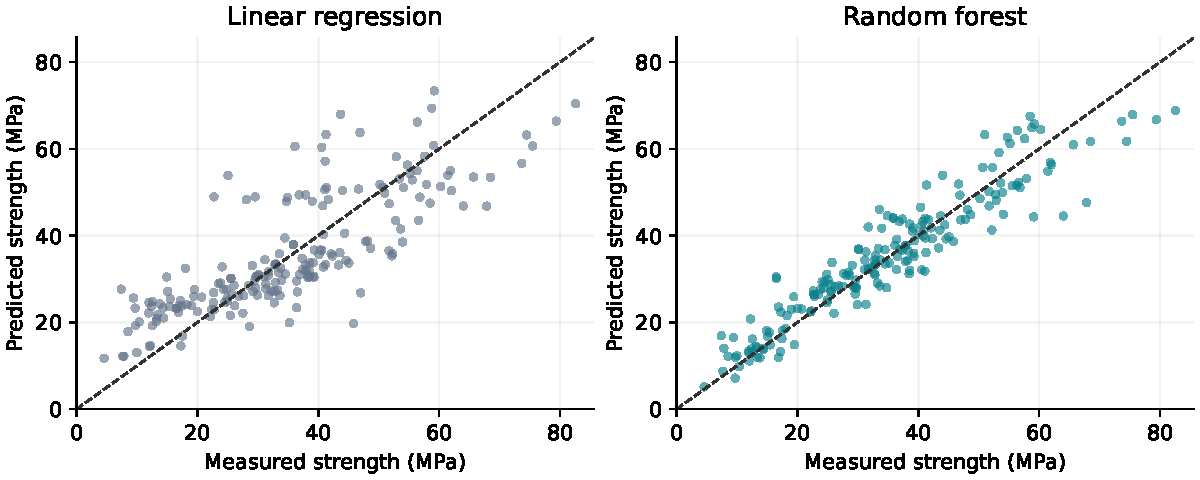
\includegraphics[width=0.90\linewidth]{../results/predictions.pdf}
\caption{Measured versus predicted strength for 195 held-out records. The
dashed line denotes perfect prediction. Both panels use identical units.}
\label{fig:pred}
\end{figure}

The forest's predictions are generally closer to the identity line
(Figure~\ref{fig:pred}), although visible deviations remain. Its RMSE exceeds
its MAE, indicating that larger errors contribute disproportionately to squared
error. An average error of 4.23 MPa may be useful for preliminary screening, but
is not a demonstrated engineering acceptance criterion. The tuned forest's CV
score is a selection score; an unbiased nested-CV estimate was not computed.
The test set provides a separate evaluation for the selected configuration.

\section{Conclusions and Reflection}
For this fixed grouped split, a modest random forest provides better predictions
than a linear baseline while remaining inexpensive to train on a CPU. The
exercise illustrates that evaluation design matters alongside model choice:
keeping repeated mix proportions together makes the test more relevant to
previously unseen exact mixes. A simple baseline also makes the added value of
the learned model measurable.

The main limitation is the scope of the data and grouping. Exact ingredient
equality does not separate near-identical mixes or establish independence between
laboratories; source identifiers and detailed curing conditions are unavailable
in the input table. Removing exact duplicates may also remove indistinguishable
replicate measurements. Results come from a single held-out group split, without
external validation or predictive uncertainty intervals. The forest does not
enforce physical constraints and should not be trusted to extrapolate beyond
the observed materials or ages.

Next steps are repeated group-based evaluation, validation on independently
collected experiments, and calibrated prediction intervals. These would help
establish when the predictor can support mix screening and when further
experimental evidence is needed.

\subsection*{Reproducibility and Disclosures}
The project supplies pinned dependencies, data attribution, scripts, split
assignments, tuning results, a saved model and example inputs. The README gives
training and inference commands. The run used Python 3.14.8 and scikit-learn
1.9.1 with seed 42. No pretrained models were used. OpenAI ChatGPT/Codex assisted
with design, coding, execution, documentation and report preparation. The author
independently reran the supplied training and inference scripts on a local
computer and reproduced the reported metrics and example predictions.

\begin{thebibliography}{9}\small
\bibitem{uci} I.-C. Yeh. \emph{Concrete Compressive Strength} [Dataset].
UCI Machine Learning Repository, 1998.
\url{https://doi.org/10.24432/C5PK67}. License: CC BY 4.0.
\bibitem{sklearn} F. Pedregosa et al. Scikit-learn: Machine Learning in Python.
\emph{Journal of Machine Learning Research}, 12:2825--2830, 2011.
\url{https://jmlr.org/papers/v12/pedregosa11a.html}.
\end{thebibliography}
\end{document}
